% This document holds the main content of the talk. It is included in
% the two global documumetns `Presentation.tex` and `Handout.tex` that
% are used to create the actual presentation as well as a two on one
% collated handout of the slides.
%
% All real content has to go to _this_ file!
%
% Last change: <Thu, 2018/05/24 12:59:11 arwagner l00slwagner.desy.de>
%
\mode<handout>{%
    \usepackage{pgf}
    \usepackage{pgfpages}
    \pgfpagesuselayout{2 on 1}[a4paper,border shrink=5mm]
}
\mode<presentation>{%
    \usetheme{DESY}
}
% Setup for Beamer
\usepackage{hyperxmp}
% \usepackage[pdfa]{hyperref}
\usepackage{luatextra}
\usepackage{wasysym}
\usepackage{eurosym}
\usepackage{bookmark}
\usepackage{graphicx}
\usepackage{fontspec}

% Force beamer to use Arial. Without this it will fall back to
% Libertine in all ``normal'' text areas. It seems they are not easily
% accessible from the templates.
\usefonttheme{professionalfonts} % using non standard fonts for beamer
\setmainfont[Mapping=tex-text]{Arial}
\setsansfont[Mapping=tex-text]{Arial}

%% Force Arial for math as well like strict CD.
%% However, usually TeX defaults just look way better
% \usepackage{unicode-math}
% \setmathfont{Arial} % for math symbols, can be any other OpenType math font
% \setmathfont[range=\mathup]  {Arial}
% \setmathfont[range=\mathbfup]{Arial Bold}
% \setmathfont[range=\mathbfit]{Arial Bold Italic}
% \setmathfont[range=\mathit]  {Arial Italic}

\usepackage[ngerman,english]{babel}
\usepackage{xspace}
\usepackage{tikz}
\usepackage{fancyvrb}
\tikzset{%
  every overlay node/.style={%
    %draw=black,fill=white,rounded corners,anchor=north west,
    draw=fzjlightblue,fill=fzjgray30,rounded corners,anchor=north west,
  },
}
% Usage:
% \tikzoverlay at (-1cm,-5cm) {content};
% or
% \tikzoverlay[text width=5cm] at (-1cm,-5cm) {content};
\def\tikzoverlay{%
   \tikz[baseline,overlay]\node[every overlay node]
}%

% General new commands an macros
\renewcommand{\emph}[1]{\structure{#1}}

\newcommand{\link}[2]{\href{#1}{~#2}}

\newcommand{\jointwo}{\href{http://join2.de}{\textbf{JOIN$^2$}\xspace}}

\newcommand{\BibTeX}{Bib\TeX}

\newcommand{\Inspec}{{\texttt{Inspec}}\xspace}
\newcommand{\WoS}{{\texttt{Web of Science}}\xspace}
\newcommand{\Scopus}{\texttt{Scopus}\xspace}
\newcommand{\arxiv}{{\texttt{arXiv.org}}\xspace}
\newcommand{\pubmed}{{\texttt{pubmed}}\xspace}

\newcommand{\JabRef}{\link{http://jabref.sf.net}{JabRef}\xspace}
\newcommand{\Companion}[1]{\textit{\link{http://julib.fz-juelich.de/uhtbin/field-search-sort/001/PBYR/213964}{\LaTeX{} Companion}, #1}\xspace}
\newcommand{\pkg}[1]{\emph{\texttt{#1}}\xspace}

\newcommand{\neutralino}{\ensuremath{\tilde{\chi}^0}\xspace}

% general colour definitions
\newcommand{\smallgray}[1]{{\tiny\emph{#1}}}

\newcommand{\idR}{i.~d.~R.\xspace}
\newcommand{\va}{v.~a.\xspace}
\newcommand{\sa}{s.~a.\xspace}
\newcommand{\zB}{z.~B.\xspace}
\newcommand{\zT}{z.~T.\xspace}
\newcommand{\eg}{e.~g.\xspace}

\newcommand{\bs}[1]{\texttt{$\backslash$#1}}
\newcommand{\command}[2]{\texttt{\bs{#1}\{#2\}}}

\newcommand{\invenio}{\href{http://invenio-software.org}{\raisebox{-0.5em}{\includegraphics[height=1.5em]{pictures/Logo_invenio}}}}
\newcommand{\github}{\href{http://github.com}{%
	\raisebox{-1em}{\includegraphics[height=2.0em]{pictures/Octocat}}%
	\raisebox{-0.5em}{\includegraphics[height=1.5em]{pictures/GitHub_Logo}}}}

\newcommand{\newitem}{\raisebox{-0.7ex}{\includegraphics[height=3ex]{img/new_icon}}}
\newcommand{\newicon}{\raisebox{-1.1ex}{\includegraphics[height=4ex]{img/new_icon}}}
\newcommand{\verytiny}[1]{{\fontsize{3}{4}\selectfont{#1}}}

\newcommand{\DESYWord}{\raisebox{-5px}{
\includegraphics[height=3.5ex]{img/DESY_Word}}\hspace*{0.2em}}

\newcommand{\MailTo}[1]{\href{mailto:#1}{#1}}
\newcommand{\DOIlink}[1]{\href{https://doi.org/#1}{\emph{#1}}}
\newcommand{\ORCiD}[1]{
\includegraphics[height=1.5ex]{img/orcid}\,\href{https://www.orcid.org/#1}{#1}}

%%--%% % http://tex.stackexchange.com/questions/16447/beamer-top-aligning-columns-within-a-top-aligned-fram
\makeatletter
\newenvironment{topitemize}{%
   \setlength{\topsep}{0pt}
   \setlength{\partopsep}{0pt}
   \renewcommand*{\@listi}{\leftmargin\leftmargini \parsep\z@ \topsep\z@ \itemsep\z@}
   \let\@listI\@listi
   \itemize
}{\enditemize}
\makeatother

%------------------- Begin of edit -----------------------------------
%
% Adopt the follwing values according to your needs.
%
% Note: improving metadata also improves visibility. Time spent here
% might pay of later. Search engines love keywords, abstracts and
% sensible titles.
%
%     Make sure to submit your talk to the publications database
%         to get a DOI, to make it citable and OpenAccess!
%
\newcommand{\TITLE}{Unfolding technique \\ for the ttbar $e-\mu$ analysis \\ via Machine Learning \\ (deep neural network)}               % Title of talk
\newcommand{\SUBTITLE}{Unfolding the leading jet pt distribution; supervised by Thorsten Kuhl \& Yichen Li at DESY Zeuthen}              % Subtitle
\newcommand{\AUTHOR}{Luiza Adelina Ciucu}        % your name
\newcommand{\EMAIL}{luiza.adelina.ciucu@cern.ch} % your email
%\newcommand{\ORCID}{0000--0001--9846--5516}   % your ORCiD
%\newcommand{\PHONE}{+49--40--8998--1758}      % your phone number
\newcommand{\GROUP}{ATLAS group at University of Geneva}          % your group
\newcommand{\URL}{http://dpnc.unige.ch/atlas/index_en.shtml}     % your groups page
%\newcommand{\DOI}{10.3204/PUBDB-20YY-nnnn}    % submit and release in pubdb to get a DOI
\newcommand{\INSTITUTE}{University of Geneva} % not used in CD 2018
\newcommand{\CITY}{Zeuthen}                      % City of talk
\newcommand{\DATE}{02.09.2019}                % Date of Talk

% To improve visibility - add metadata to the PDF
% - Add sensible keywords describing the topic
% - Add the abstract (one line, no breaks it is just for indexing)
% - Adopt the licence of your work

\hypersetup{%
	pdfkeywords        = {keyword} {keyword} {keyword},
	pdfsubject         = {Abstract},
	pdfcopyright       = {CC-BY},
	pdflicenseurl      = {http://creativecommons.org/licenses/by/4.0/},
	%% pdfcopyright       = {CC-BY-NC-SA},
	%% pdflicenseurl      = {http://creativecommons.org/licenses/by-nc-sa/4.0/},
	pdftitle           = {\TITLE}
	pdfcreator         = {\AUTHOR},
	pdfcaptionwriter   = {\AUTHOR},
	pdfcontactaddress  = {Notkestraße 85},
	pdfcontactcity     = {Hamburg},
	pdfcontactpostcode = {22607},
	pdfcontactcountry  = {Germany},
	pdfcontactemail    = {\EMAIL},
	pdfcontacturl      = {\URL},
	pdflang            = {en},
	bookmarksopen      = true,
	bookmarksopenlevel = 3,
	hypertexnames      = false,
	linktocpage        = true,
	plainpages         = false,
	breaklinks
}

%------------------- End of edit -------------------------------------

% Derive internal values from above data

\author{\AUTHOR}
\title{\TITLE}
\subtitle{\SUBTITLE}
\institute{}  % not used by DESY CD 2018
\date{\CITY, \DATE}



%---------------------------------------------------------------------

\begin{document}

\maketitle

% Add a licencse statement to all pages. Adopt this if any other
% licences is used!

%-% CC-BY-NC-SA 4
%-% \setbeamertemplate{slide counter}[showall][]
%-% \setbeamertemplate{footer element1}{%
%-%     \href{http://creativecommons.org/licenses/by-nc-sa/4.0/}{
\includegraphics[height=3ex]{img/CCBYNCSA}}
%-% }

% CC-BY 4, current suggetion for scientific content
\setbeamertemplate{slide counter}[showall][]
\setbeamertemplate{footer element1}{%
    \href{http://creativecommons.org/licenses/by/4.0/}{
\includegraphics[height=3ex]{img/CCBY}}
}

\begin{frame}{Measuring the top-quark properties is key to test the validity of the SM. The LHC is a top-quark factory.}
\centering
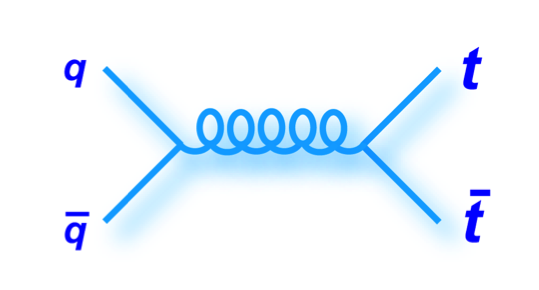
\includegraphics[height=0.25\textheight]{./plots/ttbar_1.png}
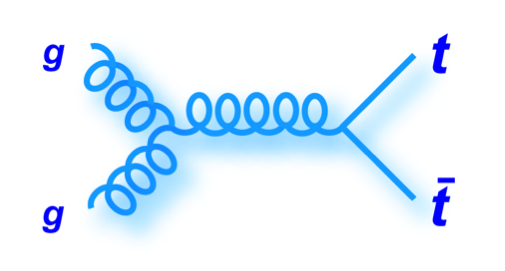
\includegraphics[height=0.25\textheight]{./plots/ttbar_2.png}
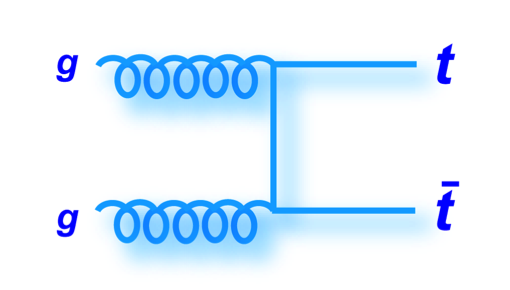
\includegraphics[height=0.25\textheight]{./plots/ttbar_3.png}
\begin{enumerate}
\item[o] The top quark is the heaviest elementary particle $\rightarrow$ largest Yukawa coupling.
\end{enumerate}
\centering
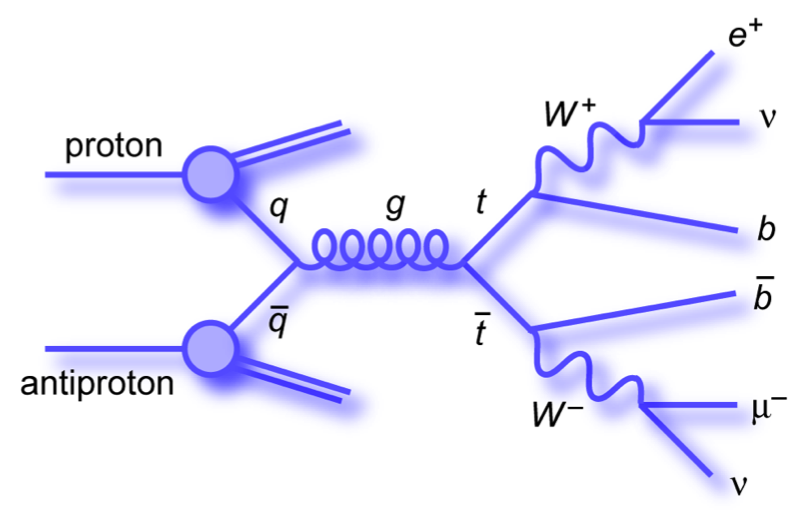
\includegraphics[height=0.3\textheight]{./plots/ttbar_4.png}
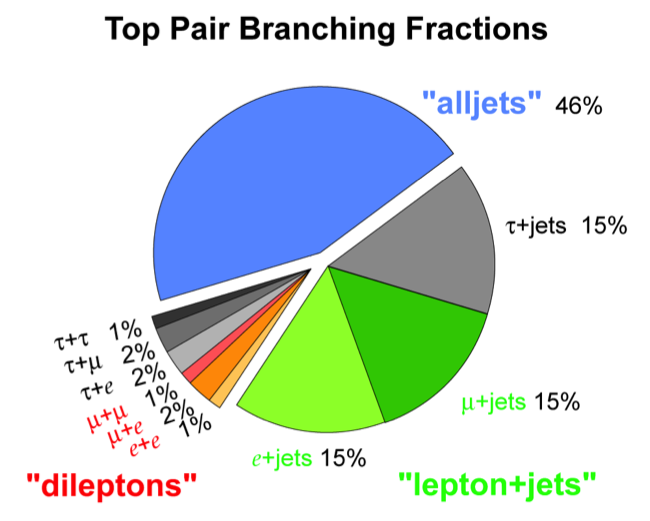
\includegraphics[height=0.3\textheight]{./plots/ttbar_5.png}
\begin{enumerate}
\item[o] Our analysis is top-quark pair-production in $e-\mu$ (2\% of ttbar).
\end{enumerate}
\end{frame}
\clearpage


\begin{frame} {Theoretical simulation vs. experimental analysis}
\begin{enumerate}
\item[o] Theoretical simulation: generated (truth) are known $\rightarrow$ observed (reco).
\item[o] Experimental analysis: observed (reco) are known $\rightarrow$ truth (nature)
\end{enumerate}
\centering
\includegraphics[height=0.53\textheight]{../output_20GeV/NN_plot1D_train_jetPt_truth_reco.pdf}
\includegraphics[height=0.53\textheight]{../output_20GeV/NN_plot1D_test_jetPt_truth_reco.pdf}
\begin{enumerate}
\item[o] The shapes of the distributions of the truth and reco observables for the training of the unfolding are very similar, but not identical (especially in the first bins). 
\end{enumerate}
\end{frame}
\clearpage


\begin{frame} {The 2D histogram of the migration matrix}
\begin{enumerate}
\item[o] The migration matrix between truth and reco is used in the traditional unfolding.
\item[o] Unfolding = inferring the generated (truth) from the observed (reconstructed).
\end{enumerate}
\centering
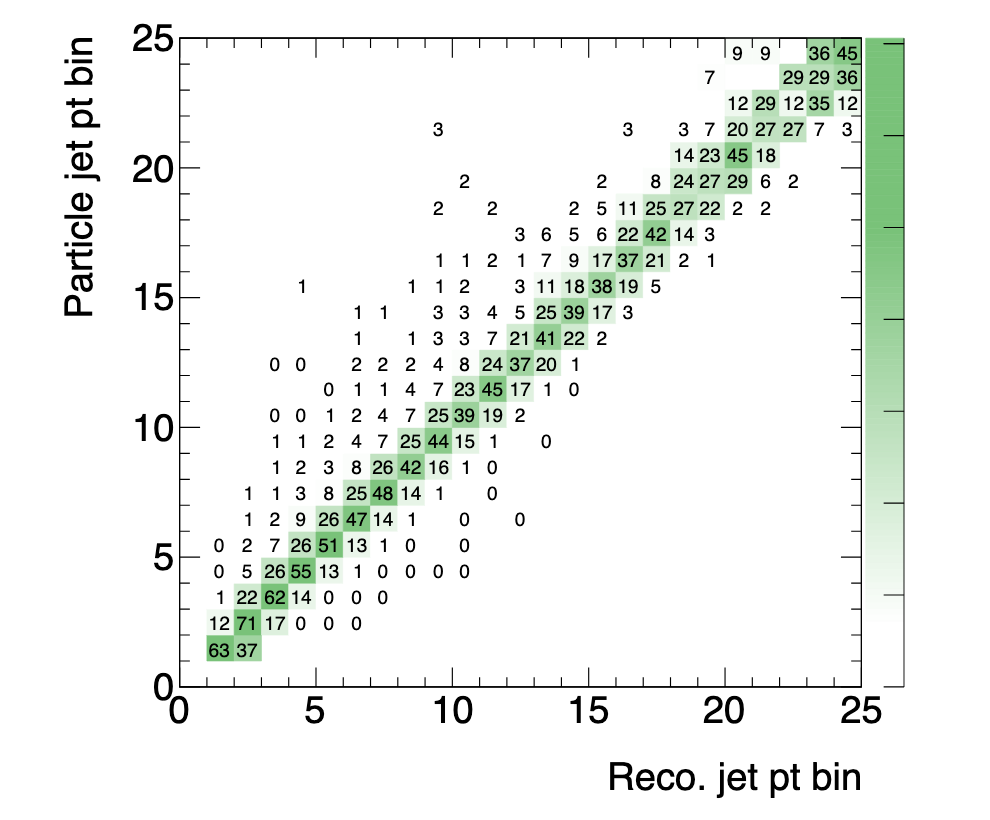
\includegraphics[height=0.42\textheight]{./plots/jetPt_migration_matrix.png}
\begin{enumerate}
\item[o] Plot from the same data, from the \href{http://www.desy.de/~liyichen/Unfolding.pdf}{report of Yichen Li}. The number in a cell represents the probability of an event in the truth bin i to be reconstructed in a reco bin j.
\item[o] The more diagonalizable matrix, the easier unfolding will be.
\item[o] Events are migrating from one truth bin to other bins for reco, and vice-versa.
\end{enumerate}
\end{frame}
\clearpage


\begin{frame}{A new approach: use machine learning to \emph{learn} how to unfold observed (reco) to true (generated).}
\begin{enumerate}
\item[o] \href{https://arxiv.org/pdf/1712.01814.pdf}{arXiv:1712:01814}
\end{enumerate}
\centering

\includegraphics[height=0.7\textheight]{./plots/PaperToyData.png}
\end{frame}
\clearpage

\begin{frame}{Two unfolding methods: traditional and ML.}
\begin{enumerate}
\item[o] Traditional: binned migration matrix with only one variable.
\item[o] Machine learning: a continuous function of several variables.
\end{enumerate}
\centering
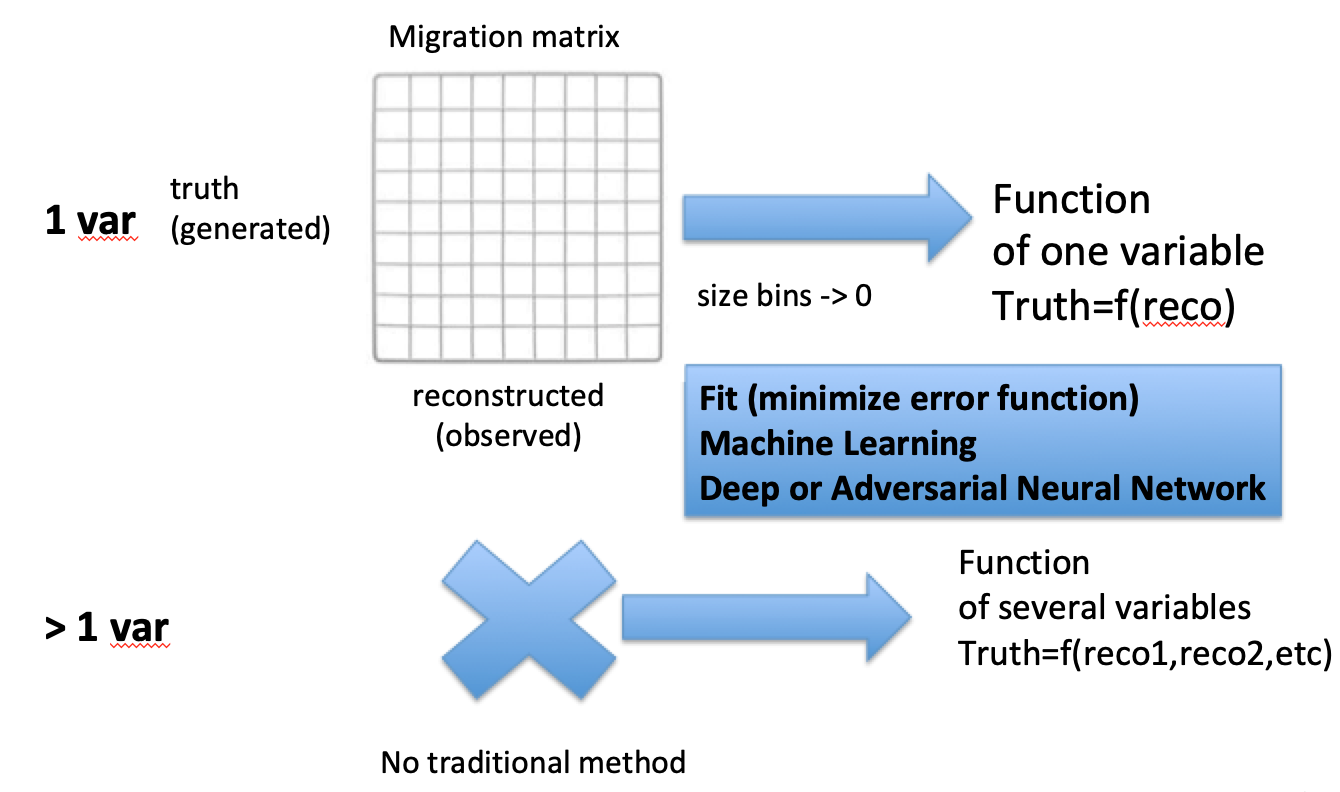
\includegraphics[height=0.70\textheight]{./plots/Unfolding_Traditional_ML.png}
\end{frame}
\clearpage

\begin{frame}{Physics problem: index of truth jet pt = f (reco jet pt) = ?}
\centering
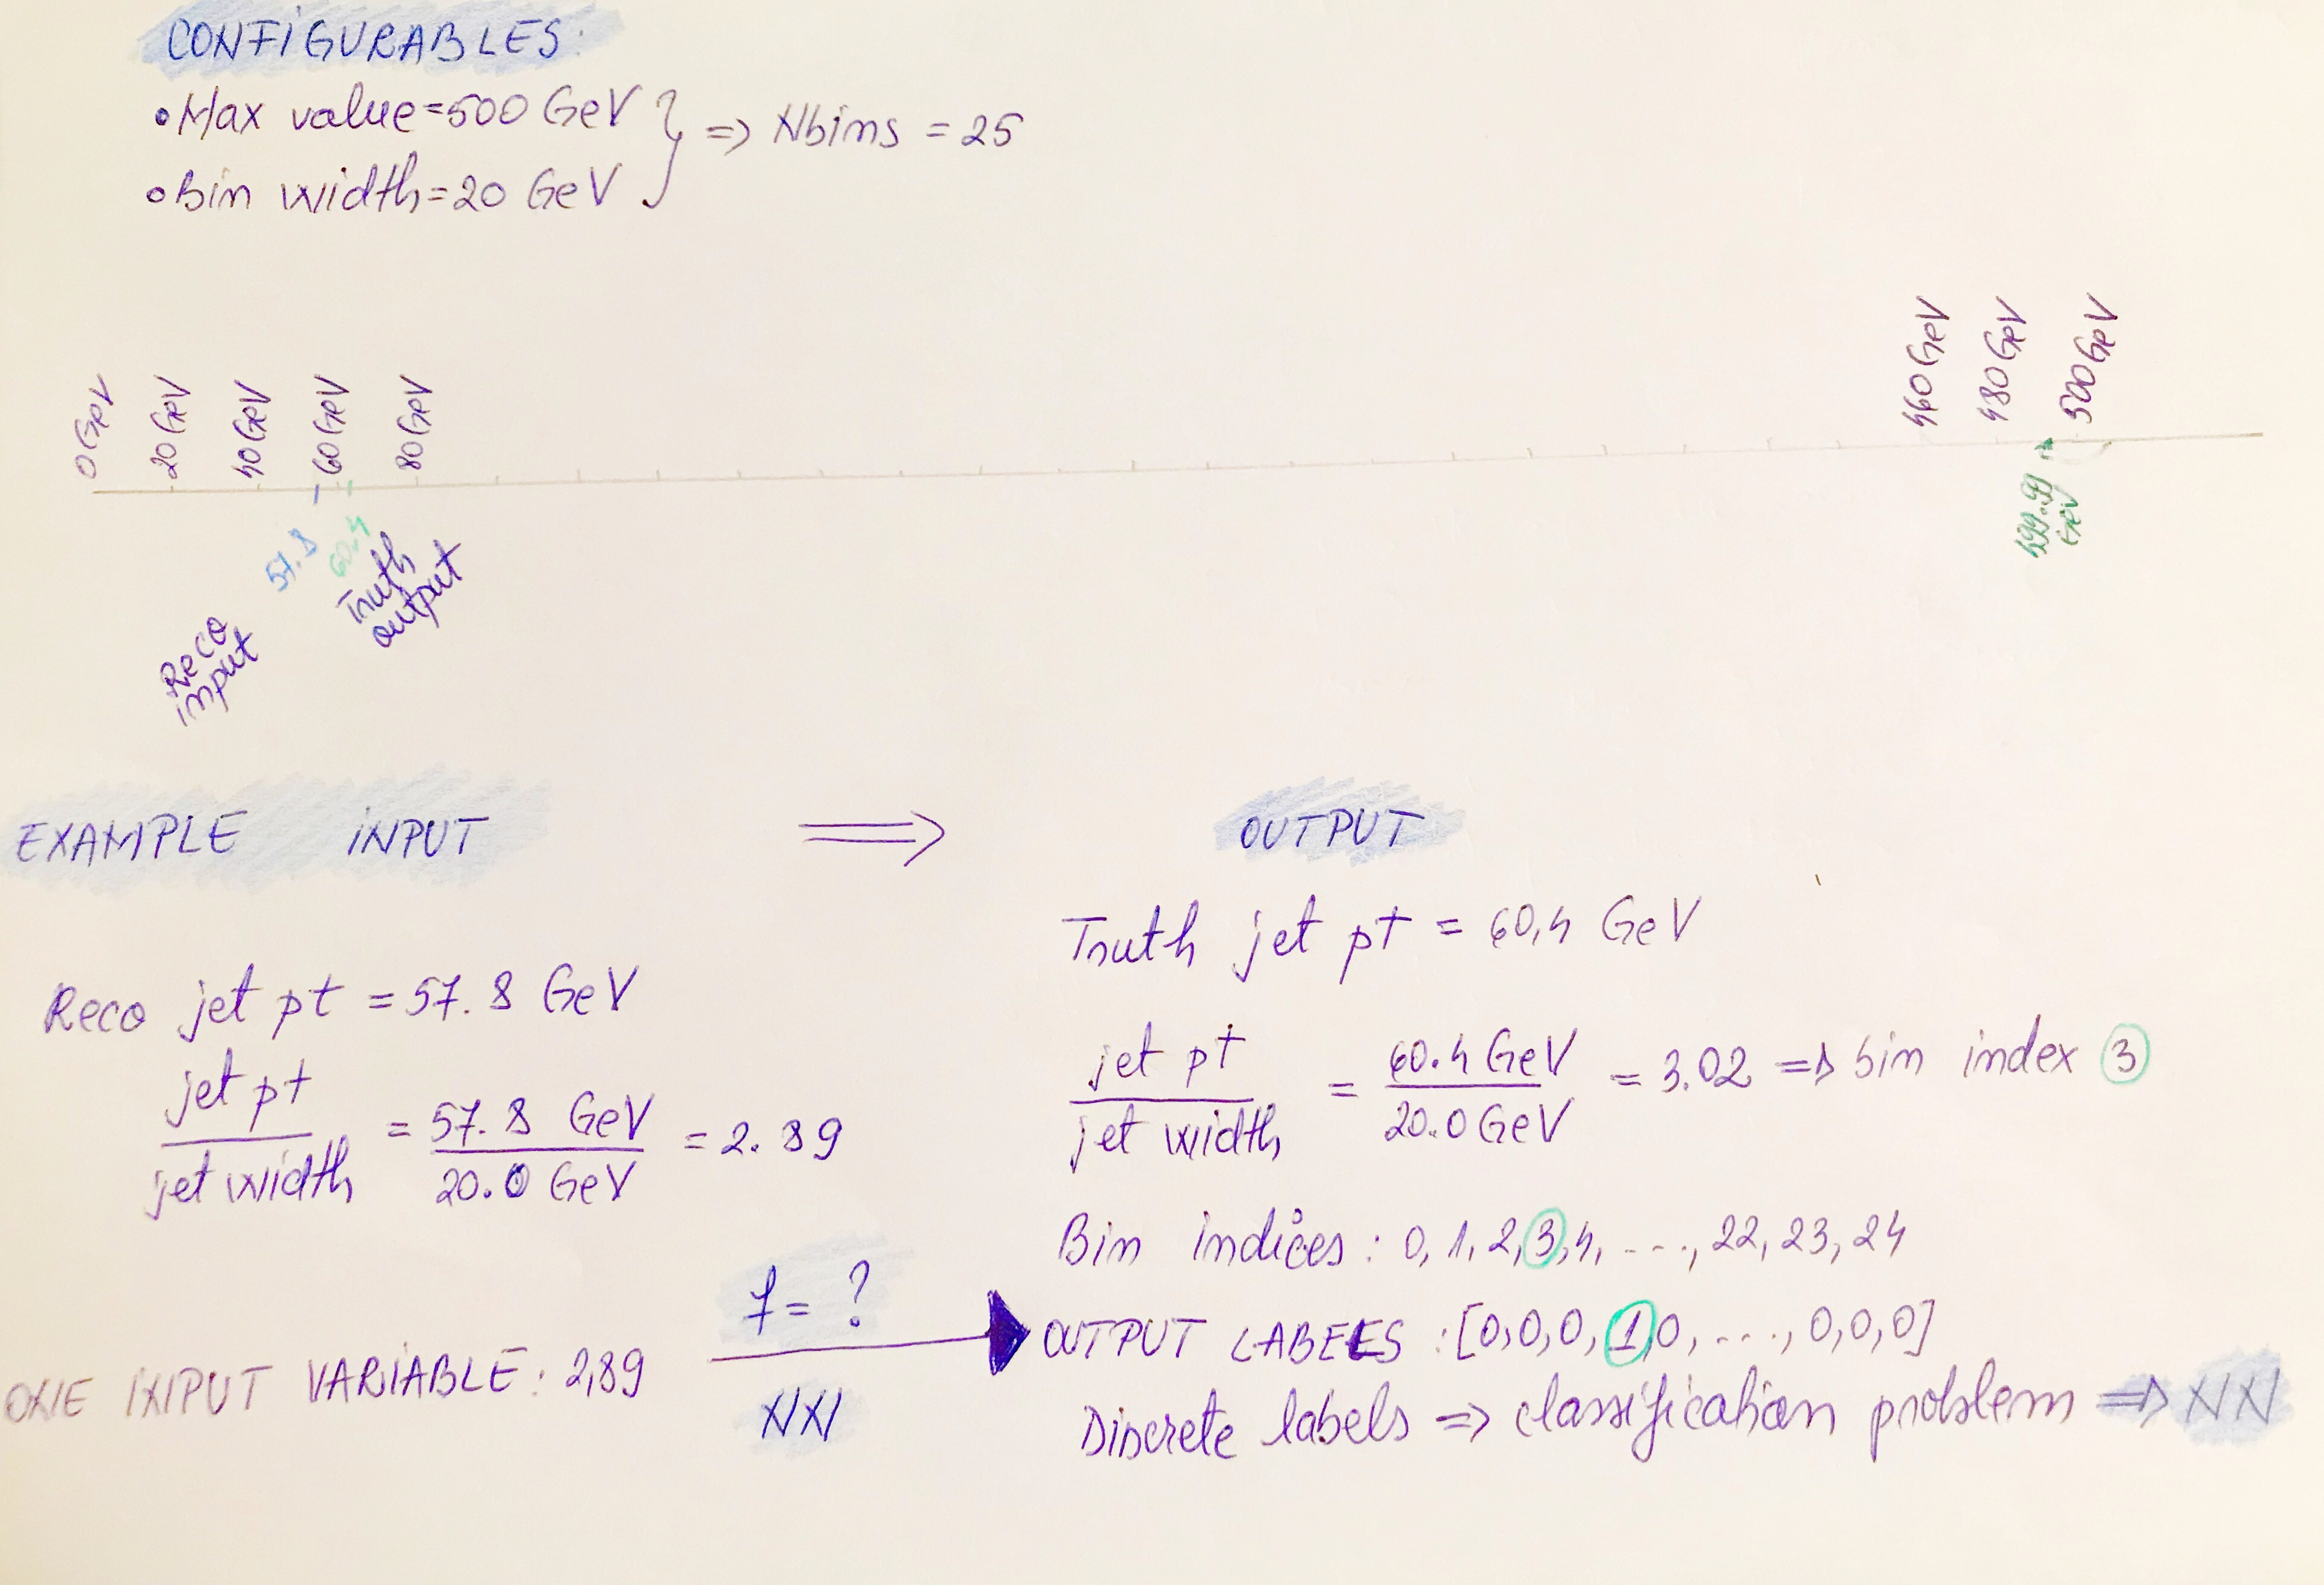
\includegraphics[height=0.80\textheight]{./plots/PhysicsProblem.jpg}
\end{frame}
\clearpage

\begin{frame}{The solution is using these NN architectures.}
\centering
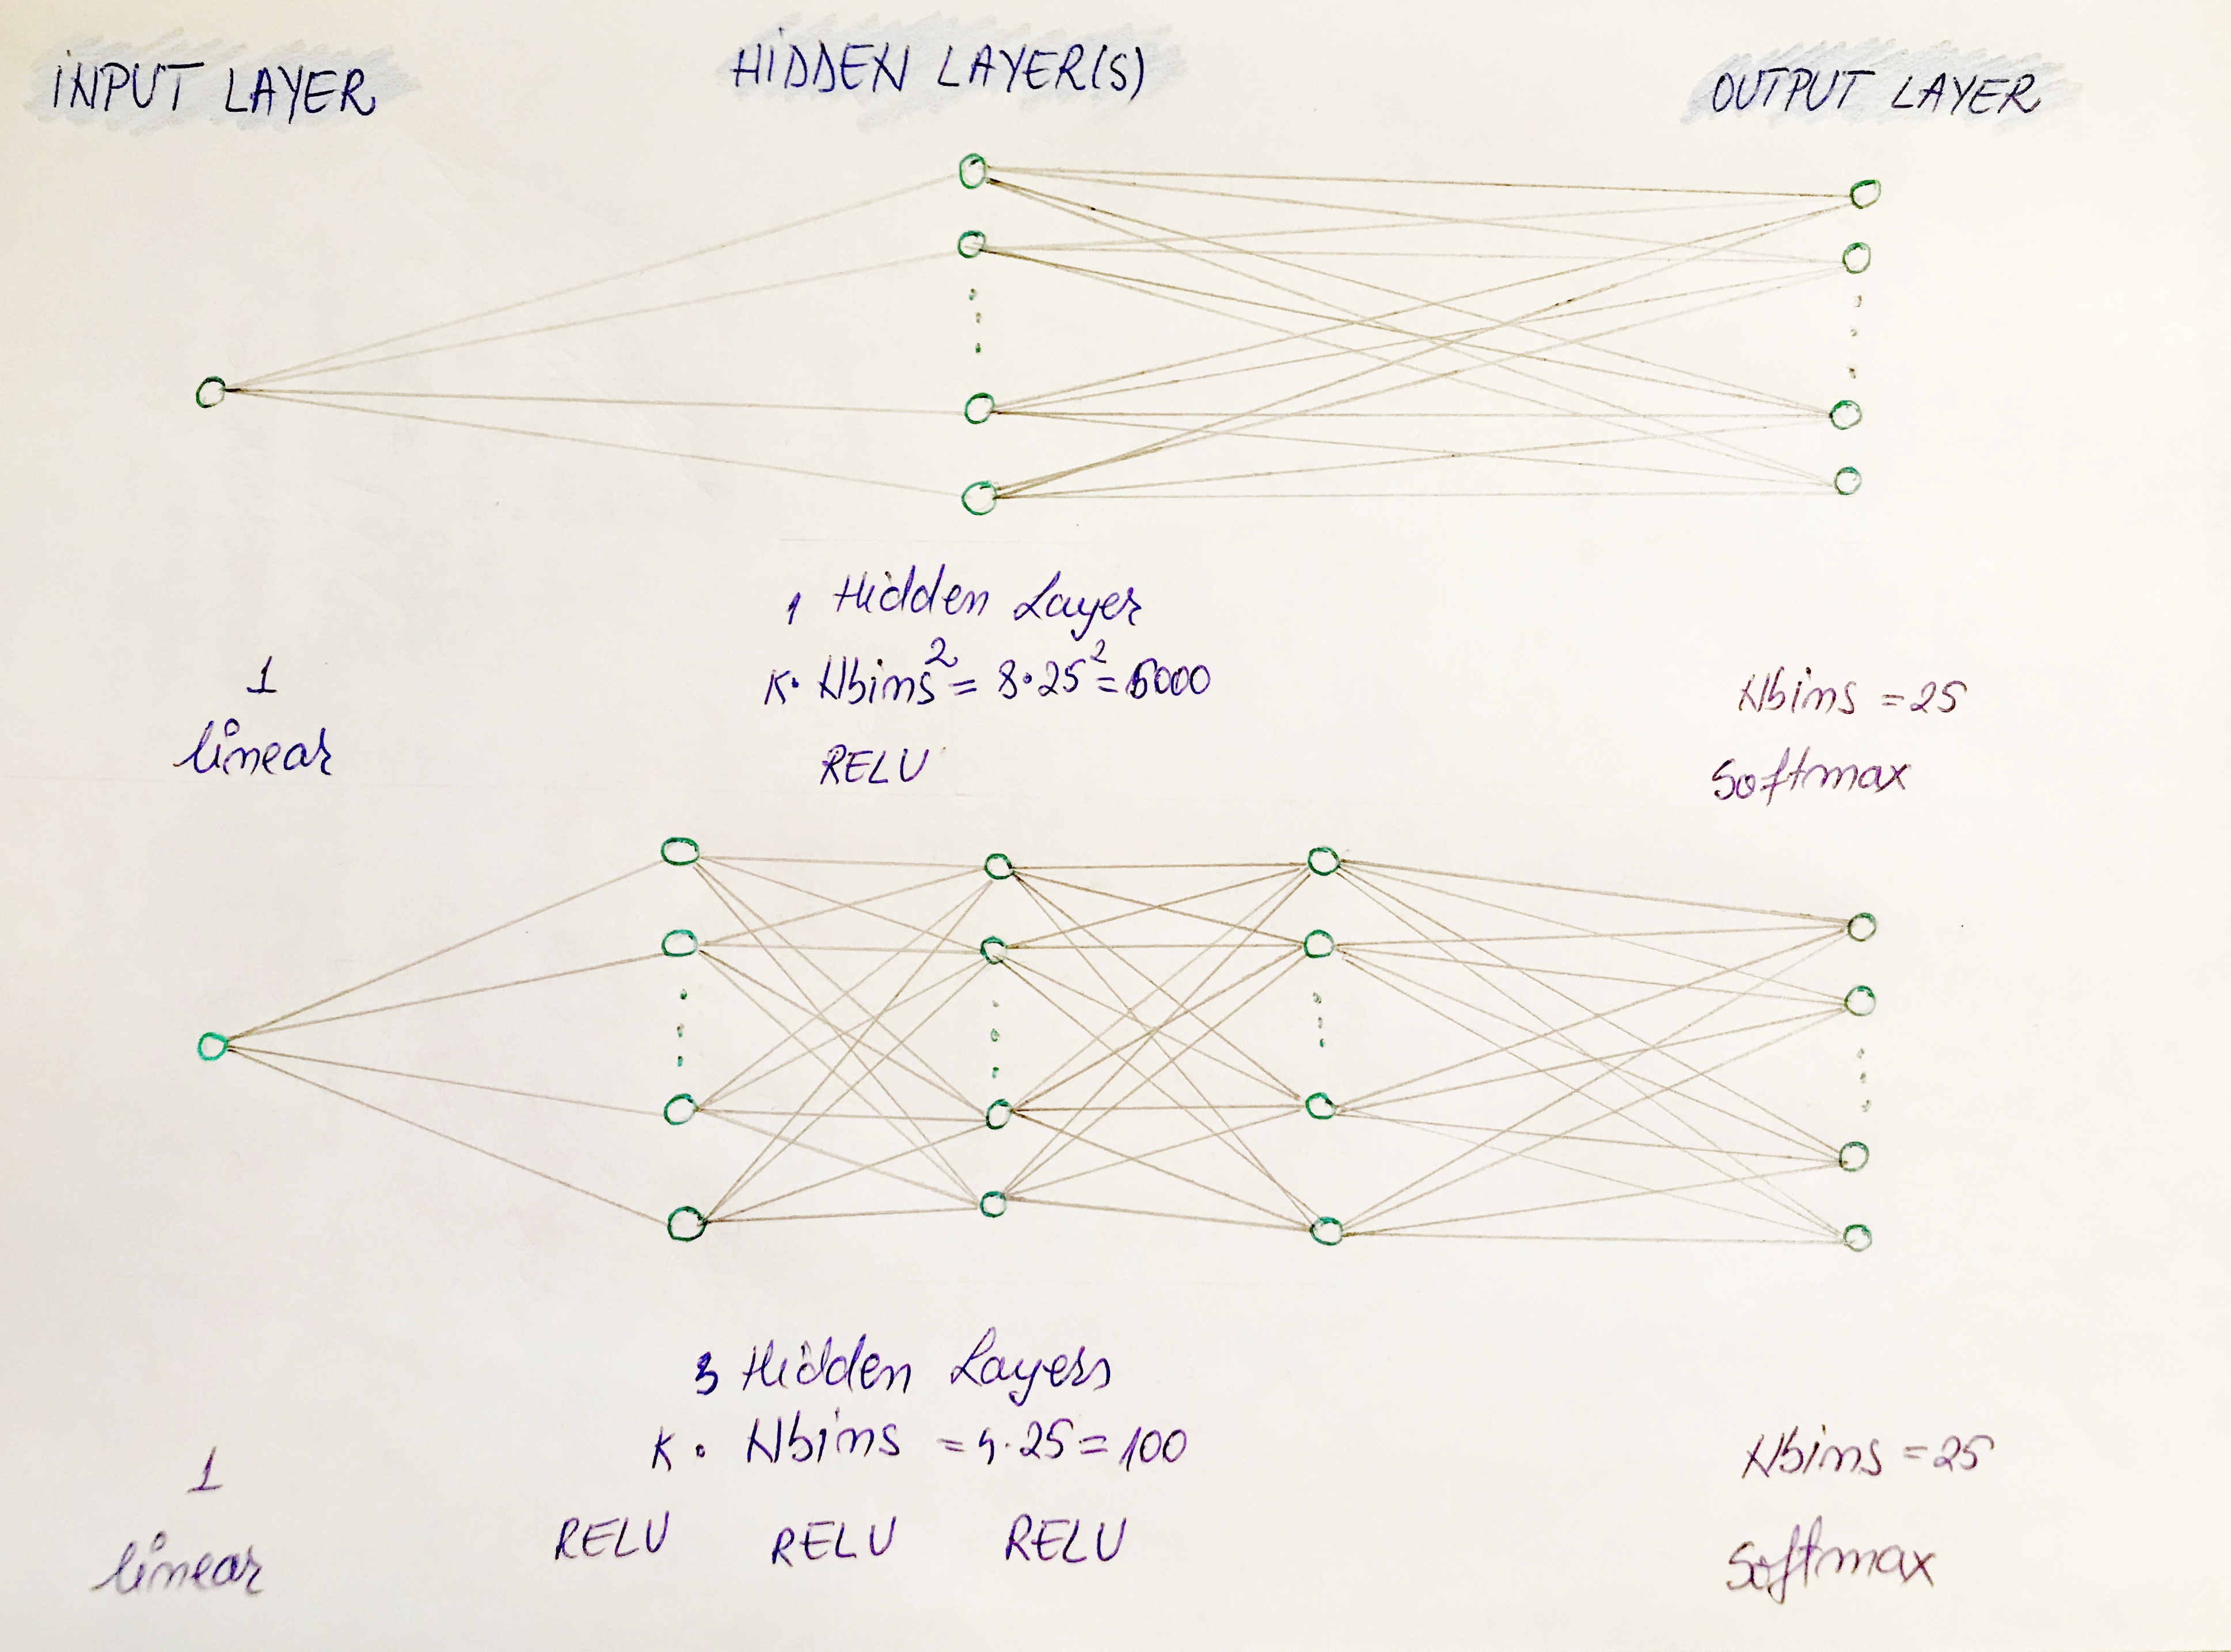
\includegraphics[height=0.80\textheight]{./plots/NNArchitecture.jpg}
\end{frame}
\clearpage

\begin{frame}{The NN is implemented in TensorFlow, via Keras, in Python.}
\centering

\includegraphics[height=0.25\textheight]{./plots/TensorFlow_Keras.png}

\includegraphics[height=0.25\textheight]{./plots/Python.png}
\begin{enumerate}
\item[o] Ran the DNN software for unfolding by DESY Hamburg.
\item[o] Ran on lxplus using the ML software docker image via singularity.
\item[o] Read the ROOT file via the uproot package.
\item[o] Trained  the NNs in Python using Keras and TensorFlow.
\end{enumerate}
\ \\
\ \\
\begin{enumerate}
\item[o] Fine tuned the NN hyper parameters for our ROOT data sample.
\item[o] One NN training is the first step of the iterative unfolding procedure. 
\end{enumerate}
\end{frame}
\clearpage

\begin{frame}{Summary of the physics and NN choices}
\begin{table}[h!]
\begin{enumerate}
\item[o] One file with 43076 events (and leading jets). Half (21538) in training, half in testing. 
\item[o] jet pt: range=0-500 GeV, bin width=20 GeV, number of bins = 500/20 = 25.
\item[o] Chose the NN training hyper-parameters by changing one at a time while keeping the other constant, and choosing those with largest accuracy and smallest loss values.
\end{enumerate}
  \resizebox{\textwidth}{!}{
    \begin{tabular}{|l|l|l|} % <-- Alignments: 1st column left, 2nd middle and 3rd right, with vertical lines in between
      \hline
      \textbf{Choice} & \textbf{Old NN (toy data example)} & \textbf{New NN (my best choice)}\\
      \hline
      number of nodes per input layer & 1 & 1 \\
      number of nodes per output layer & ${\rm Nbins}=25$ & ${\rm Nbins}=25$ \\
      Number of hidden layers & 1 & 3 \\
      ${\rm k}$ & 8 & 4 \\
      Number of nodes per layer & ${\rm k}\cdot {\rm Nbins}^2=5000$ & ${\rm k}\cdot {\rm Nbins}=100$ \\
      activation function input & linear & linear \\
      activation function hidden & ReLU & ReLU \\
      activation function output & softmax & softmax \\
      batch size & 1000 & 200 \\
      number of epochs & 150 & 150 \\
      \hline
    \end{tabular}
  }
\end{table}
\end{frame}
\clearpage

\begin{frame}{Two figures of merit to optimise the NN hyper-parameters}
\begin{enumerate}
\item[o] The accuracy: the larger, the better (left: old NN; right: new NN).
\end{enumerate}
\centering
\includegraphics[height=0.28\textheight]{../output_20GeV/NN_plot1D_optionTrainTest_accuracy_NN_l_A1_k_8_e_150_b_1000.pdf}
\includegraphics[height=0.28\textheight]{../output_20GeV/NN_plot1D_optionTrainTest_accuracy_NN_l_B3_k_4_e_150_b_200.pdf}\\
\begin{enumerate}
\item[o] The loss (error) value: the smaller, the better (left: old NN; right: new NN).
\end{enumerate}
\centering
\includegraphics[height=0.28\textheight]{../output_20GeV/NN_plot1D_optionTrainTest_loss_NN_l_A1_k_8_e_150_b_1000.pdf}
\includegraphics[height=0.28\textheight]{../output_20GeV/NN_plot1D_optionTrainTest_loss_NN_l_B3_k_4_e_150_b_200.pdf}\\
\begin{enumerate}
\item[o] Overlaid \textcolor{cyan}{train} and \textcolor{magenta}{test} are very similar $\rightarrow$ we did not overtrain the NNs. 
\end{enumerate}
\end{frame}
\clearpage

\begin{frame}{Overlaying the two NN architectures: \textcolor{red}{old} and \textcolor{OliveGreen}{new}. }
\begin{enumerate}
\item[o] The accuracy: the larger, the better (left: train; right: test).
\end{enumerate}
\centering
\includegraphics[height=0.28\textheight]{../output_20GeV/NN_plot1D_train_accuracy_NN_final.pdf}
\includegraphics[height=0.28\textheight]{../output_20GeV/NN_plot1D_test_accuracy_NN_final.pdf}\\
\begin{enumerate}
\item[o] The loss (error) value: the smaller, the better (left: train; right: test).
\end{enumerate}
\centering
\includegraphics[height=0.28\textheight]{../output_20GeV/NN_plot1D_train_loss_NN_final.pdf}
\includegraphics[height=0.28\textheight]{../output_20GeV/NN_plot1D_test_loss_NN_final.pdf}\\
\begin{enumerate}
\item[o] The \textcolor{OliveGreen}{new} NN architecture outperforms the \textcolor{red}{old} one.
\end{enumerate}
\end{frame}
\clearpage

\begin{frame}{The jet pt distribution as the index of the jet pt bin.}
\begin{enumerate}
\item[o] True output (generated, truth) vs input (reconstructed). Used in traditional unfolding.
\end{enumerate}
\centering
\includegraphics[height=0.27\textheight]{../output_20GeV/NN_plot1D_train_jetPtBin_NN_noTrained.pdf}
\includegraphics[height=0.27\textheight]{../output_20GeV/NN_plot1D_test_jetPtBin_NN_noTrained.pdf}
\begin{enumerate}
\item[o] The true output vs the predicted unfolded output by each NN architecture.
\item[o] The \textcolor{OliveGreen}{new} NN architecture is closer to the \textcolor{blue}{true output} than the \textcolor{red}{old} one.
\end{enumerate}
\centering
\includegraphics[height=0.27\textheight]{../output_20GeV/NN_plot1D_train_jetPtBin_NN_final.pdf}
\includegraphics[height=0.27\textheight]{../output_20GeV/NN_plot1D_test_jetPtBin_NN_final.pdf}
\end{frame}
\clearpage

\begin{frame}{The predicted NN output minus the true output.}
\begin{enumerate}
\item[o] Both outputs are integers, representing bin indices, $\rightarrow$ difference = also integer.
\item[o] The greater the count at zero difference, the better.
\item[o] Top: train, bottom: test. Left to right, bin widths of 10, 20, 50, 100 GeV.
\item[o] The smaller the binWidth, the better is the \textcolor{OliveGreen}{new} NN architecture relative to the \textcolor{red}{old} one.
\end{enumerate}
\centering
\includegraphics[height=0.25\textheight]{../output_10GeV/NN_plot1D_train_outputPredictedMinusTrue_NN_final.pdf}
\includegraphics[height=0.25\textheight]{../output_20GeV/NN_plot1D_train_outputPredictedMinusTrue_NN_final.pdf}
\includegraphics[height=0.25\textheight]{../output_50GeV/NN_plot1D_train_outputPredictedMinusTrue_NN_final.pdf}
\includegraphics[height=0.25\textheight]{../output_100GeV/NN_plot1D_train_outputPredictedMinusTrue_NN_final.pdf}\\
\includegraphics[height=0.25\textheight]{../output_10GeV/NN_plot1D_test_outputPredictedMinusTrue_NN_final.pdf}
\includegraphics[height=0.25\textheight]{../output_20GeV/NN_plot1D_test_outputPredictedMinusTrue_NN_final.pdf}
\includegraphics[height=0.25\textheight]{../output_50GeV/NN_plot1D_test_outputPredictedMinusTrue_NN_final.pdf}
\includegraphics[height=0.25\textheight]{../output_100GeV/NN_plot1D_test_outputPredictedMinusTrue_NN_final.pdf}
\end{frame}
\clearpage

\begin{frame}{The 2D histogram migration matrix of the index of the jet pt}
\begin{enumerate}
\item[o] The closer to a diagonal matrix, the better.
\item[o] Top: train, Bottom: test.
\item[o] Left to right: input, \textcolor{red}{old} NN output, \textcolor{OliveGreen}{new} NN output vs true output. 
\end{enumerate}
\centering
\includegraphics[height=0.25\textheight]{../output_20GeV/NN_plot2D_train_outputTrue_input.pdf}
\includegraphics[height=0.25\textheight]{../output_20GeV/NN_plot2D_train_outputTrue_outputPredicted_NN_l_A1_k_8_e_150_b_1000.pdf}
\includegraphics[height=0.25\textheight]{../output_20GeV/NN_plot2D_train_outputTrue_outputPredicted_NN_l_B3_k_4_e_150_b_200.pdf}\\
\includegraphics[height=0.25\textheight]{../output_20GeV/NN_plot2D_test_outputTrue_input.pdf}
\includegraphics[height=0.25\textheight]{../output_20GeV/NN_plot2D_test_outputTrue_outputPredicted_NN_l_A1_k_8_e_150_b_1000.pdf}
\includegraphics[height=0.25\textheight]{../output_20GeV/NN_plot2D_test_outputTrue_outputPredicted_NN_l_B3_k_4_e_150_b_200.pdf}\\
\end{frame}
\clearpage

\begin{frame}{Summary and Next Steps}
\begin{enumerate}
\item[o] Studied Unfolding of the jet pt distributions in ttbar e-mu analysis.
\item[o] Bin of truth jet pt = f (reco jet pt) = ?
\item[o] Discrete output values  $\rightarrow$ classification problem $\rightarrow$ NN.
\item[o] Coded using Tensor Flow via Keras in Python.
\item[o] Followed code example with toy data in arXiv (\href{https://arxiv.org/pdf/1712.01814.pdf}{link for arXiv:1712:01814}).
\item[o] Fine tuned NN hyper-parameters and architecture for our jet data.
\item[o] The chosen NN outperforms the one from the toy data.
\item[o] The project code and report are in GitLab (\href{https://gitlab.cern.ch/lciucu/MLUnfolding/}{link}).
\end{enumerate}
\ \\
\ \\
\begin{enumerate}
\item[o] Training recursively several NNs of the found architecture.
\begin{enumerate}
\item[o] One NN training is just the first (zeroth) step in the NN unfolding method.
\end{enumerate}
\item[o] Use more data (more events and leading jets).
\item[o] Add other input variables (e.g. jet $\eta$).
\end{enumerate}
\end{frame}
\clearpage

\begin{frame}{Backup slides}
\end{frame}
\clearpage

\begin{frame}{Traditional unfolding results}
\begin{enumerate}
\item[o] Plot taken from Fig. 5 of \href{http://www.desy.de/~liyichen/Unfolding.pdf}{study by Yichen Li}.
\item[o] Traditional unfolding: iterative bayesian unfolding with 4 iterations.
\end{enumerate}
\centering
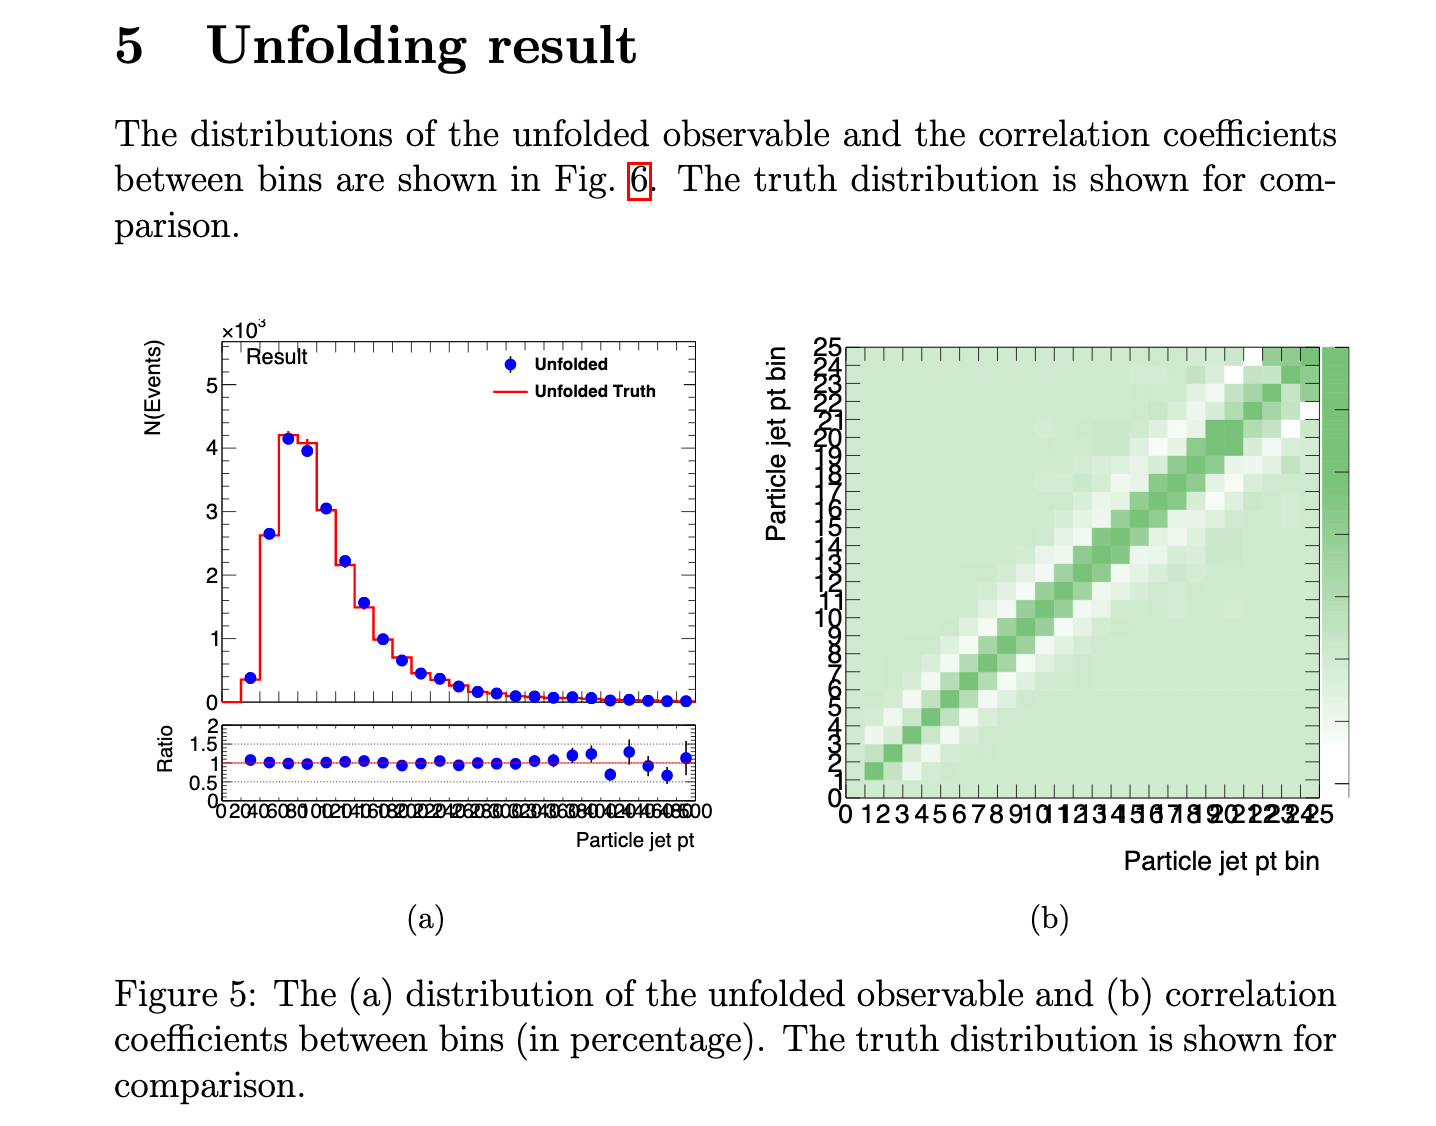
\includegraphics[height=0.65\textheight]{./plots/TraditionalUnfolding.png}
\end{frame}
\clearpage


\end{document}

%----------------------------------------------------------------------
% Add manual table of contents
% Two column example
%-% \begin{frame}
%-% \frametitle{Overview}
%-%   \begin{columns}
%-%       \begin{column}{0.4\textwidth}
%-%           \hspace*{-0.97cm}\includegraphics[height=\textheight]{img/menzel}
%-%       \end{column}
%-%       \begin{column}{0.5\textwidth}
%-%           \begin{itemize}[<+->]
%-%               \item {Section}
%-%               \item {Section}
%-%           \end{itemize}
%-%       \end{column}
%-%   \end{columns}
%-% \end{frame}

\begin{frame}
\frametitle{Overview}
  \begin{itemize}[<+->]
      \item {Section}
      \item {Section}
  \end{itemize}
\end{frame}

%----------------------------------------------------------------------
% Missuse parts as chapters according to DESY PR
\part[Part slide]{Part slide}
\makepart%

%----------------------------------------------------------------------
\section{\ldots}

% Add a sample slide with some math, some columns etc.
\begin{frame}[t,label=...]
\frametitle{Lorem ipsum}
\ldots dolor sit amet, consectetur adipiscing elit. Sed facilisis
dui vel tempor hendrerit. Fusce id sapien sit amet ligula tempor
porttitor tempus quis mi.

\[
    E_{t,ij} = \sum_{k,l} \sum_{\lambda_i, \lambda_i'}
        \rho_{\lambda_1,\lambda_1'}(e^-_1)
        \rho_{\lambda_2,\lambda_2'}(e^-_2)
        [T_{ij}^{\lambda_1\phantom{'} \lambda_2}(\neutralino_k)]
        \cdot
        [T_{ij}^{\lambda_1' \lambda_2'}(\neutralino_k)]^*
\]

% left aligned columns. Note that columns with smaller width are
% centred automatically
\begin{columns}
    \begin{column}[t]{0.48\textwidth}
    Duis autem vel eum iriure dolor in hendrerit in vulputate velit
    esse molestie consequat, vel illum dolore eu feugiat nulla
    facilisis at vero eros et accumsan\ldots
    \end{column}
    \begin{column}[t]{0.48\textwidth}
    Nam liber tempor cum soluta nobis eleifend option congue nihil
    imperdiet \ldots
    \end{column}
\end{columns}
\end{frame}


%----------------------------------------------------------------------
% Thank you page is assembled from metadata.tex
\begin{frame}
\frametitle{Thank you!}
\vfill{}
\vspace*{3.5cm}

% check %-% comments for inclusion of a QR code. This is not official
% DESY CD.

\fontsize{8}{9}\selectfont
\begin{columns}
	\hspace*{-0.8em}
	\hspace*{-1em}  % comment if QR code is inserted
	%-% \begin{column}{0.75\textwidth}
	\begin{column}{\textwidth}
		\begin{tabular}{lll}
		\textbf{Contact}&\hspace*{0.5cm} & \\
						&\hspace*{0.5cm} & \\
		\hspace*{-0.4mm}\DESYWord{}Deutsches&\hspace*{0.5cm} & \AUTHOR \\
		Elektronen-Synchrotron &\hspace*{0.5cm} \\%& \ORCiD{\ORCID}\\
							&\hspace*{0.5cm} & \GROUP  \\
							&\hspace*{0.5cm} & \MailTo{\EMAIL}\\
		www.desy.de			%&\hspace*{0.5cm} & \PHONE \\
							%&\hspace*{0.5cm} & \DOIlink{\DOI}\\
		\end{tabular}
	\end{column}
	%-% \begin{column}{0.24\textwidth}
	%-% \includegraphics[width=0.8\textwidth]{img/aw-vcf-QRCode}\\
	%-% 	{\tiny\textit{Typeset by lua\LaTeX}}
	%-% \end{column}
\end{columns}
\end{frame}

\end{document}
% Enable spell checker for vim
% setlocal spell spelllang=de
